\documentclass[10pt,letterpaper]{article}

\usepackage[margin=0.72in]{geometry}
\usepackage{amsmath,amssymb}
\usepackage{graphicx}
\usepackage{booktabs}
\usepackage{caption}
\usepackage{subcaption}
\usepackage{float}
\usepackage{enumitem}
\usepackage{microtype}
\usepackage[hidelinks]{hyperref}

\graphicspath{{figures/isotope/}}
\setlength{\parindent}{0pt}
\setlength{\parskip}{4pt}
\setlist{nosep,leftmargin=*}
\captionsetup{font=footnotesize}

\title{\vspace{-1.3cm}
Linear Stability of Electron--Hydrogen and
Electron--Deuterium Plasmas in Dipole Geometry:
A GENE Parameter Study}
\author{MAE 190 --- Research Division}
\date{November 2026}

\begin{document}
\maketitle
\vspace{-0.7cm}

\section{Objective}

This study investigates how density gradients, temperature
gradients, and ion mass affect the linear stability of
electron--ion plasmas in dipole magnetic geometry. Using the
gyrokinetic code GENE, we compare electron--hydrogen (H)
and electron--deuterium (D) plasmas while keeping the
reference normalization and other model parameters fixed.

The primary quantities of interest are the normalized
linear growth rate $\gamma$ and the difference
$\Delta\gamma=\gamma_H-\gamma_D$.
Positive growth rates indicate exponentially growing
linear perturbations; negative rates indicate decay.
The study is restricted to a fixed perpendicular
wavenumber and does not directly calculate nonlinear
turbulent transport.

\section{Numerical Setup and Parameter Scan}

GENE was compiled and tested on an Apple Silicon Mac
using the \texttt{mac\_arm64} configuration. Initial
single-case runs were used to verify execution,
diagnostic output, and the dipole-geometry setup.

The simulations were electrostatic and linear, with
two kinetic species: electrons and either hydrogen
or deuterium ions. Both species had unit normalized
density and temperature, with charges $-1$ and $+1$,
respectively. The ion mass was changed from
$m_i=1$ for hydrogen to $m_i=2$ for deuterium,
while the reference mass was held fixed at $m_{\rm ref}=1$.
The electron mass was $m_e=0.00054462$ in the same
reference units.

The common numerical configuration included
\[
\begin{gathered}
n_{k_y}=1,\quad n_z=32,\quad n_{v_\parallel}=48,
\quad n_\mu=32,\\
k_{y,\min}=0.7,\quad
N_{\rm steps}=5000,\quad
\beta=0,\quad \nu=0.01.
\end{gathered}
\]
The dipole geometry used
$r_{0,\mathrm{dipole}}=0.4$,
$I_{\mathrm{curr,dipole}}=750$, and
$c_{\mathrm{surf,dipole}}=1.2$.
Other numerical and physical settings were held
constant between the isotope cases.

The normalized density and temperature gradients
were varied independently over
\[
\mathrm{omn},\mathrm{omt}
\in\{0,\ 0.5,\ 1,\ 2,\ 3,\ 4,\ 5\}.
\]
For each case, both species were assigned the same
density-gradient and temperature-gradient parameters.
This produced $7\times7=49$ cases per isotope,
or \textbf{98 simulations in total}.

\section{GENE Growth Rates and Unresolved Cases}

For simulations satisfying GENE's linear-growth
convergence criterion, the growth rate and real
frequency were extracted from \texttt{out/omega.dat}.
Of the 98 simulations, 85 formally converged:
44 hydrogen cases and 41 deuterium cases.

The remaining 13 simulations did not meet the
convergence criterion within 5000 time steps.
These cases were concentrated in the low-gradient
region. They could not be assigned zero growth
or labeled stable merely because convergence was
not achieved. Increasing the simulation duration
had not reliably resolved this behavior, motivating
an analysis of the recorded energy evolution.

\section{Estimating Growth Rates from Free Energy}

For a linear perturbation with amplitude
$A(t)\propto e^{\gamma t}$, a positive quadratic
energy-like diagnostic evolves as
\[
W(t)\propto |A(t)|^2\propto e^{2\gamma t}.
\]
Taking the natural logarithm gives
\[
\ln W(t)=\ln W_0+2\gamma t,
\]
and therefore
\begin{equation}
\boxed{
\gamma_{\mathrm{eff}}
=\frac{1}{2}\frac{d}{dt}\ln W(t)
}
\label{eq:energygrowth}
\end{equation}

For each unresolved case, the time and total
free energy were read from columns 1 and 2
of GENE's \texttt{out/energy.dat}.
A straight line was fitted to $\ln W(t)$
over late-time windows comprising the final
50\%, 30\%, and 15\% of the recorded evolution.
Half the fitted slope was interpreted as the
effective energy-growth rate.

The final 15\% estimate was used for the
exploratory numerical values. Agreement between
different fit windows and approximately linear
late-time behavior in $\ln W$ were used to assess
the reliability of each estimate.

This method has an important limitation:
the total free energy can contain contributions
from multiple evolving modes. During mode
competition or transient evolution, its logarithmic
slope need not equal the growth rate of a single
eigenmode. Therefore, an energy-derived estimate
must not be represented as a formally converged
GENE eigenvalue.


\subsection{Convergence and Reliability Classification Criteria}

Each simulation was assigned a quality classification
using a hierarchical procedure. The classification
distinguishes solver-confirmed eigenmode convergence
from growth rates inferred through post-processing.

\begin{enumerate}[label=\textbf{\arabic*.},leftmargin=*]

\item \textbf{GENE-converged.}
A simulation was classified as converged only if
its \texttt{run.log} contained GENE's explicit
message \texttt{Linear growth rate is converged}.
The growth rate and real frequency were then
read from \texttt{out/omega.dat}.
This criterion was determined by GENE's internal
convergence test, rather than by our energy fits.
A simulation that completed its time steps without
this message was not classified as converged.

\item \textbf{Qualified energy-derived estimate.}
For a simulation without confirmed GENE convergence,
the effective growth rate was estimated from the
slope of $\ln W(t)$, divided by two.
Linear fits were calculated over the final
50\%, 30\%, and 15\% of the recorded time history.

An estimate was classified as qualified when
visual inspection showed an approximately
exponential late-time energy evolution and
the fitted slopes were sufficiently consistent
to support a representative growth rate.
These estimates are marked with an asterisk
($*$) in the heatmaps.

\item \textbf{Uncertain energy-derived estimate.}
An estimate was classified as uncertain when
the energy evolution exhibited substantial
curvature, oscillations, transient behavior,
or sensitivity to the selected fitting window.
The final-15\% slope was retained as an
exploratory estimate, but it was not considered
a reliable single-mode growth rate.
These values are marked with a dagger
($\dagger$) in the supplementary heatmaps
and omitted from the primary heatmaps.

\end{enumerate}

\textbf{Interpretation of the rubric.}
The first category is based on an explicit
solver-generated convergence result.
The distinction between qualified and uncertain
energy estimates is a post-processing judgment
based on fit-window consistency and the observed
shape of the late-time energy evolution.

No universal numerical tolerance for the
difference between the 15\%, 30\%, and 50\%
fits was established in this analysis.
Consequently, the latter two categories
should be understood as diagnostic reliability
assessments, not formal statistical confidence
levels or independently verified eigenvalues.

For a single dominant exponential mode,
the three fitted slopes should approach
the same value as transient contributions decay.
Persistent disagreement indicates that the
effective energy-growth rate remains dependent
on the observation window.

\section{Data Quality and Figure Classification}

The 98 results were separated into three categories:

\begin{center}
\begin{tabular}{lrrr}
\toprule
Classification & Hydrogen & Deuterium & Total\\
\midrule
GENE-converged & 44 & 41 & 85\\
Qualified energy estimate ($*$) & 1 & 5 & 6\\
Uncertain energy estimate ($\dagger$) & 4 & 3 & 7\\
\midrule
Total & 49 & 49 & 98\\
\bottomrule
\end{tabular}
\end{center}

The six qualified energy estimates exhibited
sufficiently consistent late-time behavior to
support cautious interpretation. The seven
uncertain estimates were affected by changing
fit slopes, oscillations, or transitional behavior.
Their numerical values are useful for exploration,
but cannot be treated as reliable eigenmode rates.

Two versions of the heatmaps were prepared.
The \emph{primary} figures show the 85 converged
rates and six qualified energy estimates, leaving
the seven uncertain values blank. The
\emph{supplementary} figures display all 98 values,
marking the uncertain estimates with $\dagger$.
Both sets retain the same normalization and
comparable color scales.

\section{Results}

\subsection{Primary Validated Heatmaps}

\begin{figure}[H]
\centering
\begin{subfigure}{0.32\linewidth}
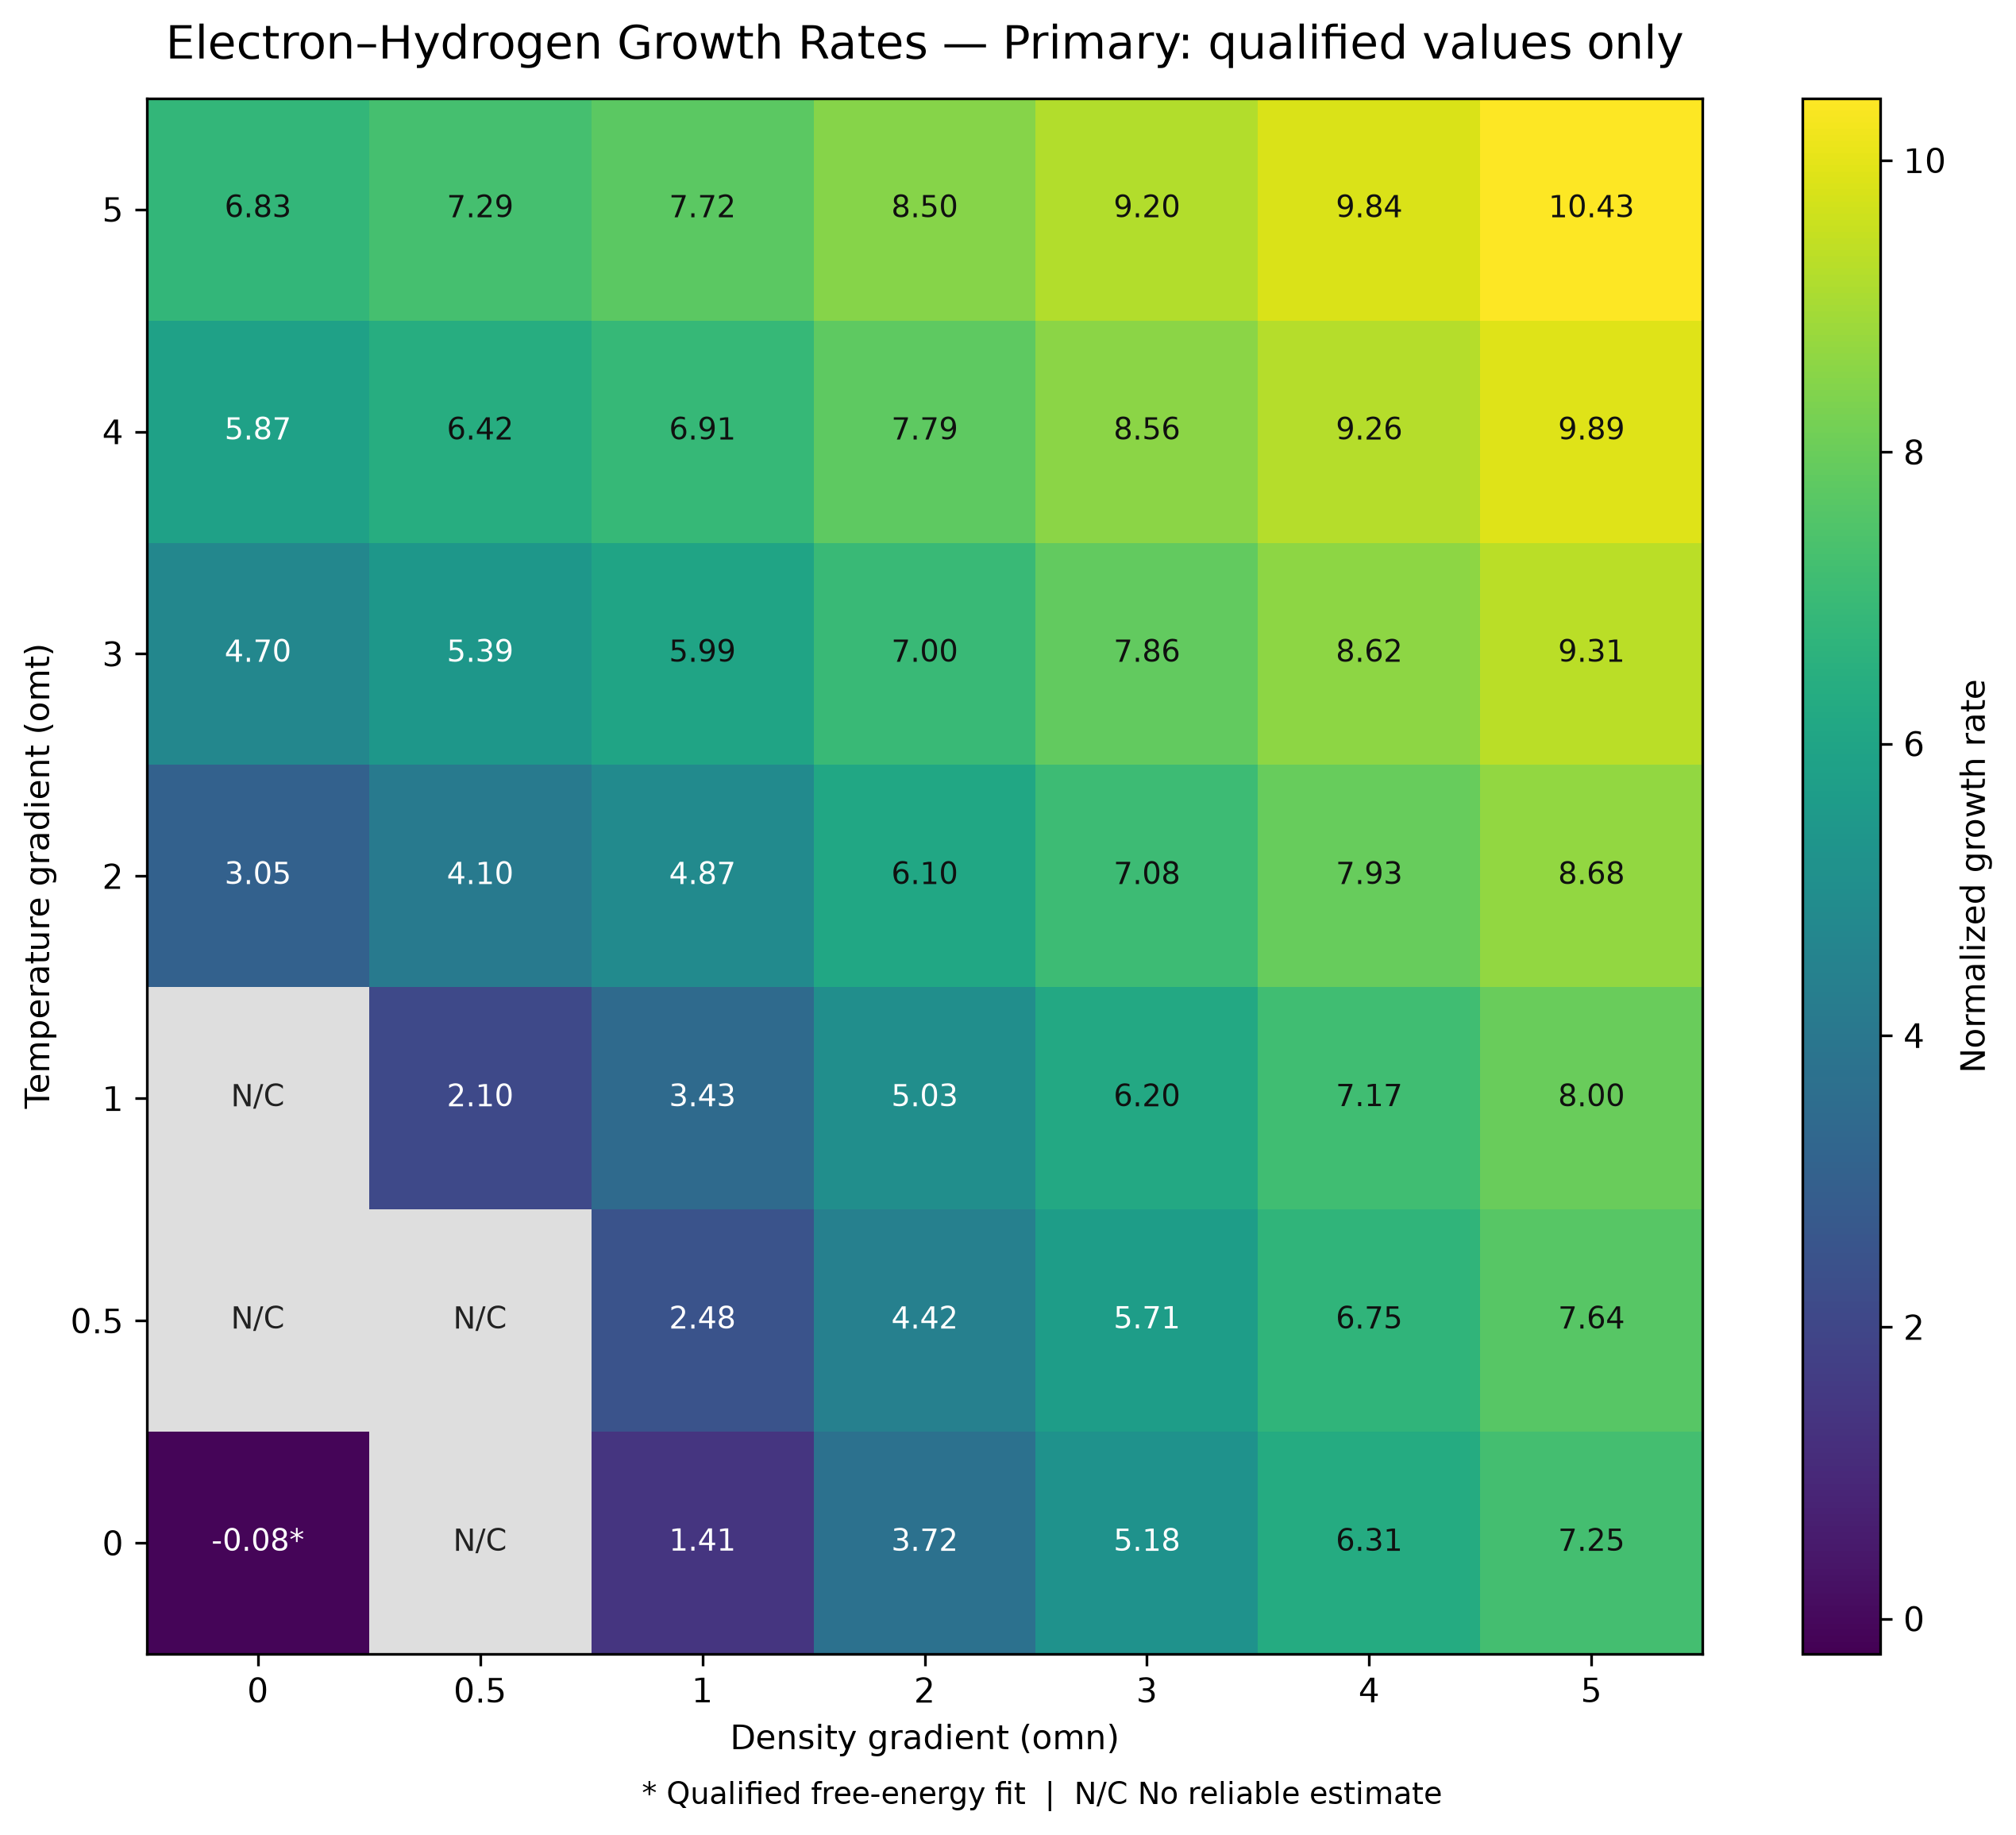
\includegraphics[width=\linewidth]{primary_validated_hydrogen.png}
\caption{Electron--hydrogen}
\end{subfigure}
\begin{subfigure}{0.32\linewidth}
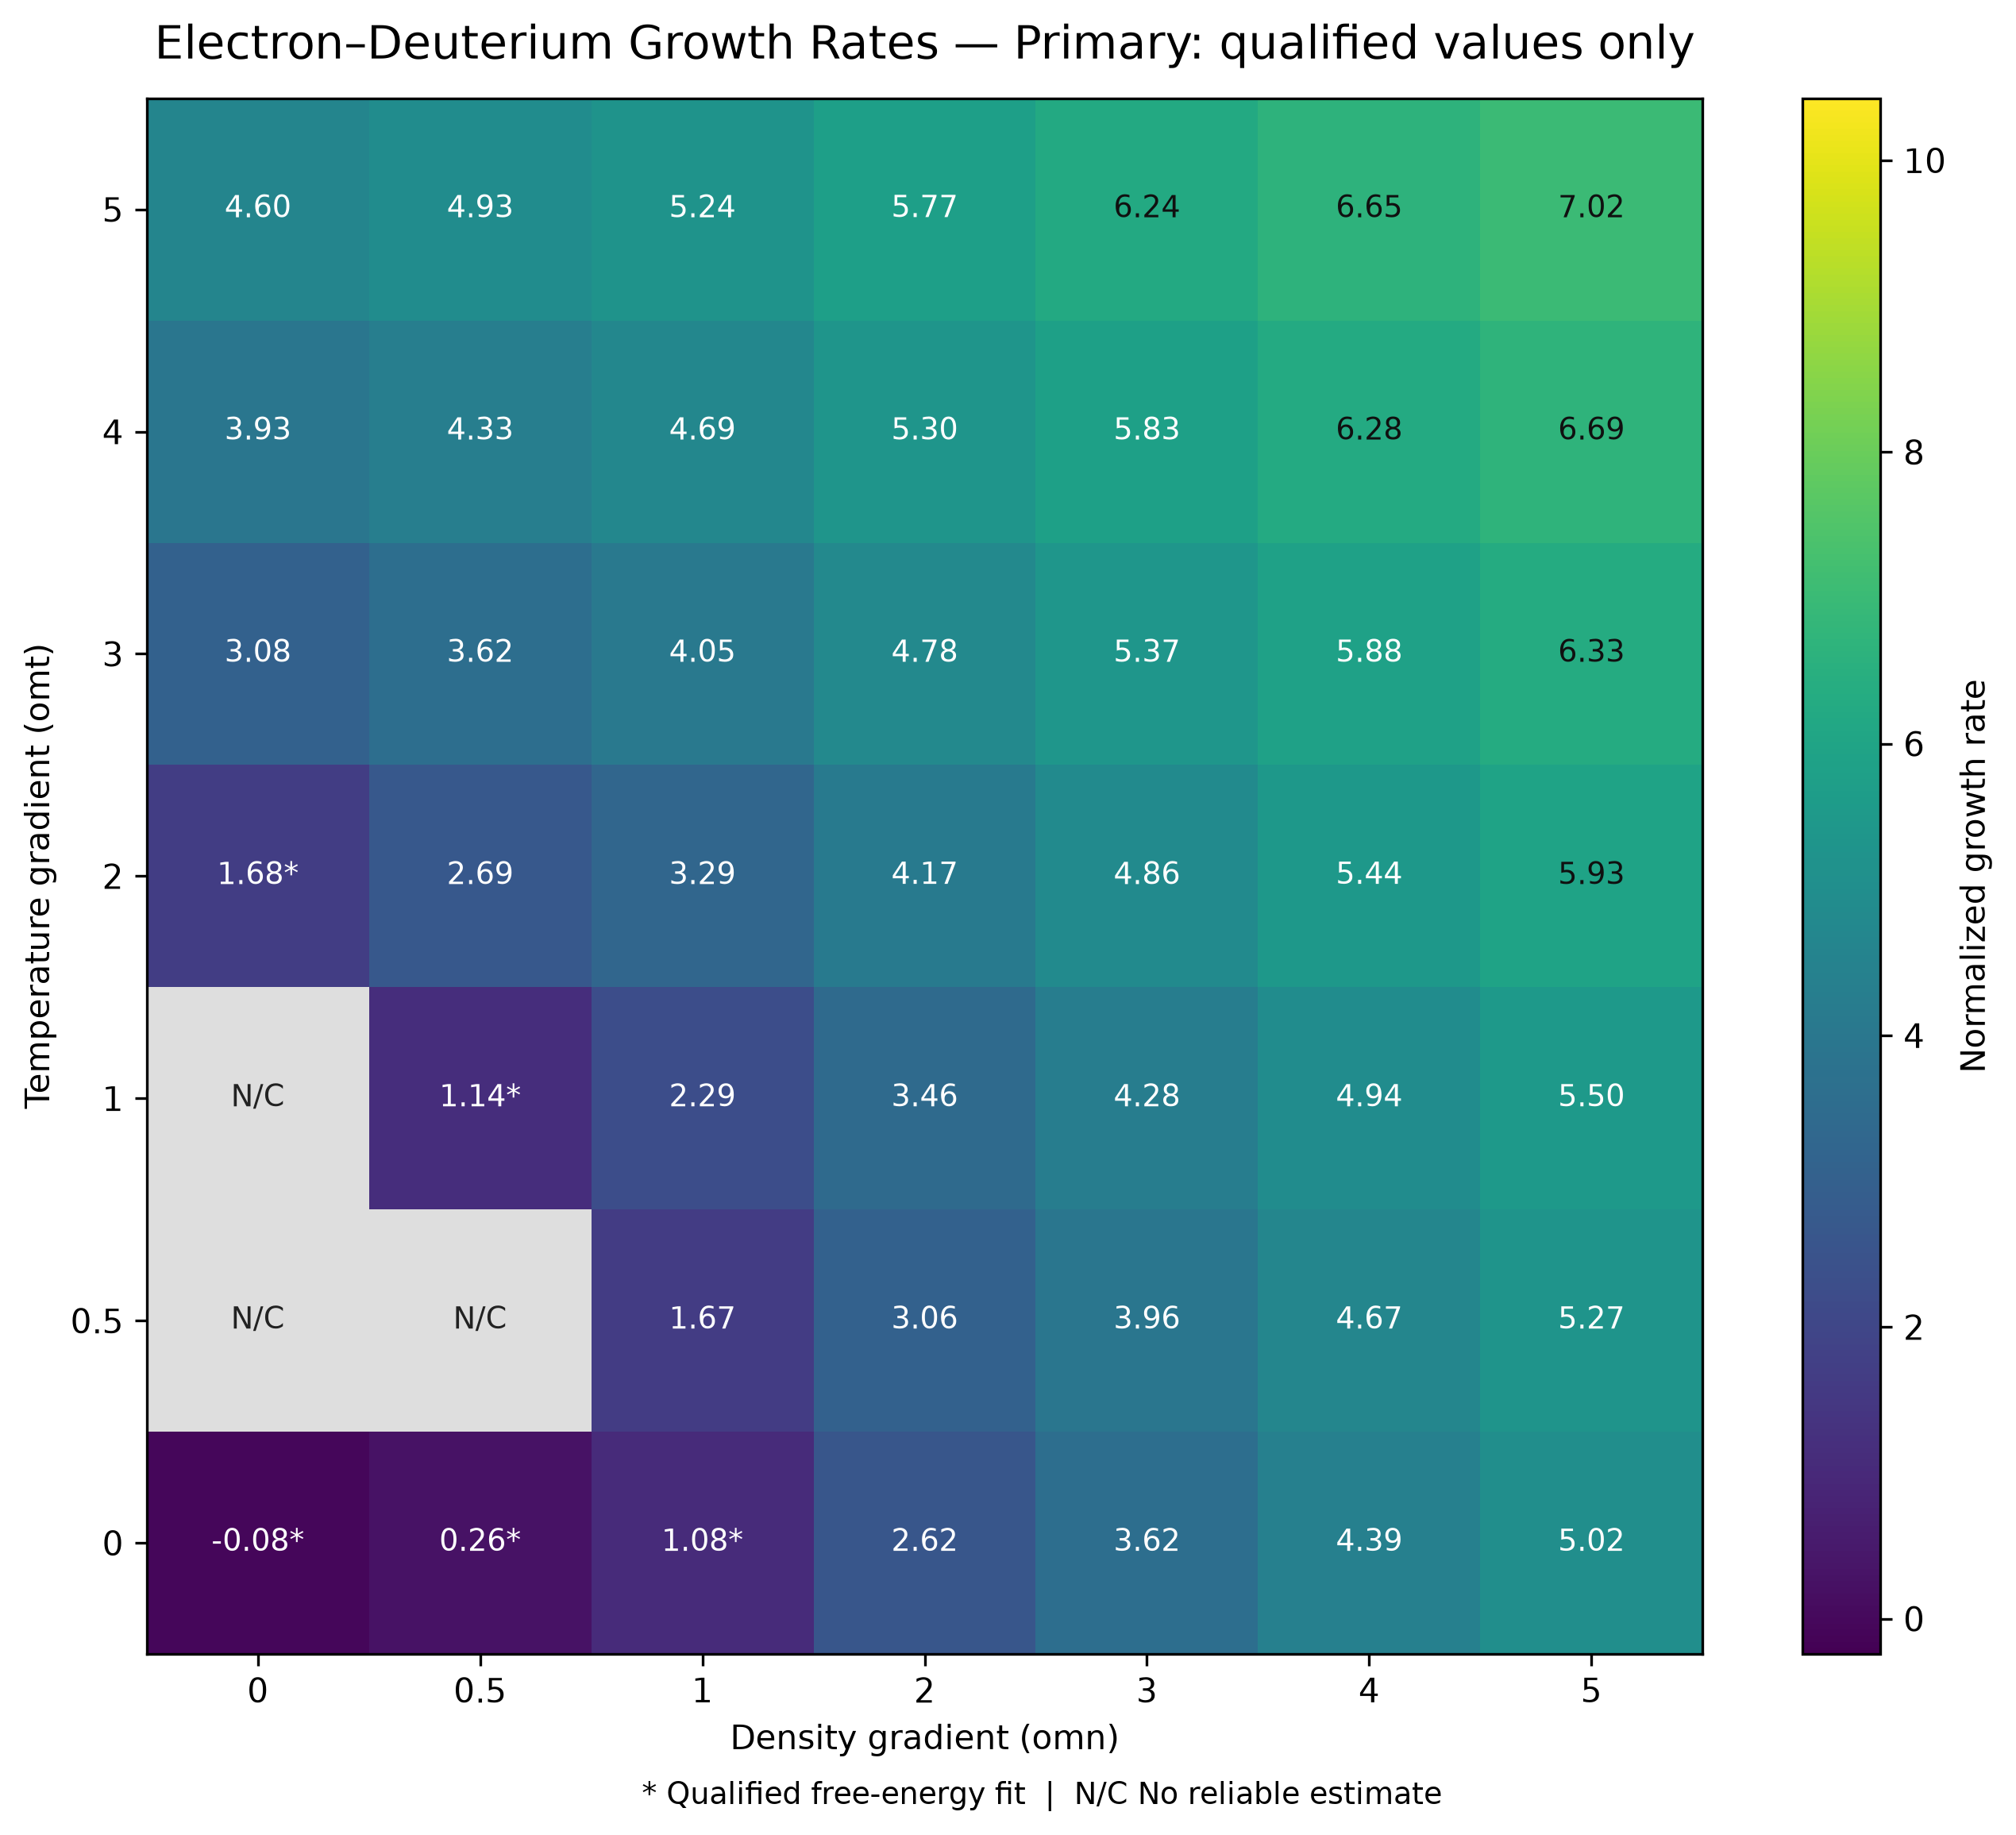
\includegraphics[width=\linewidth]{primary_validated_deuterium.png}
\caption{Electron--deuterium}
\end{subfigure}
\begin{subfigure}{0.32\linewidth}
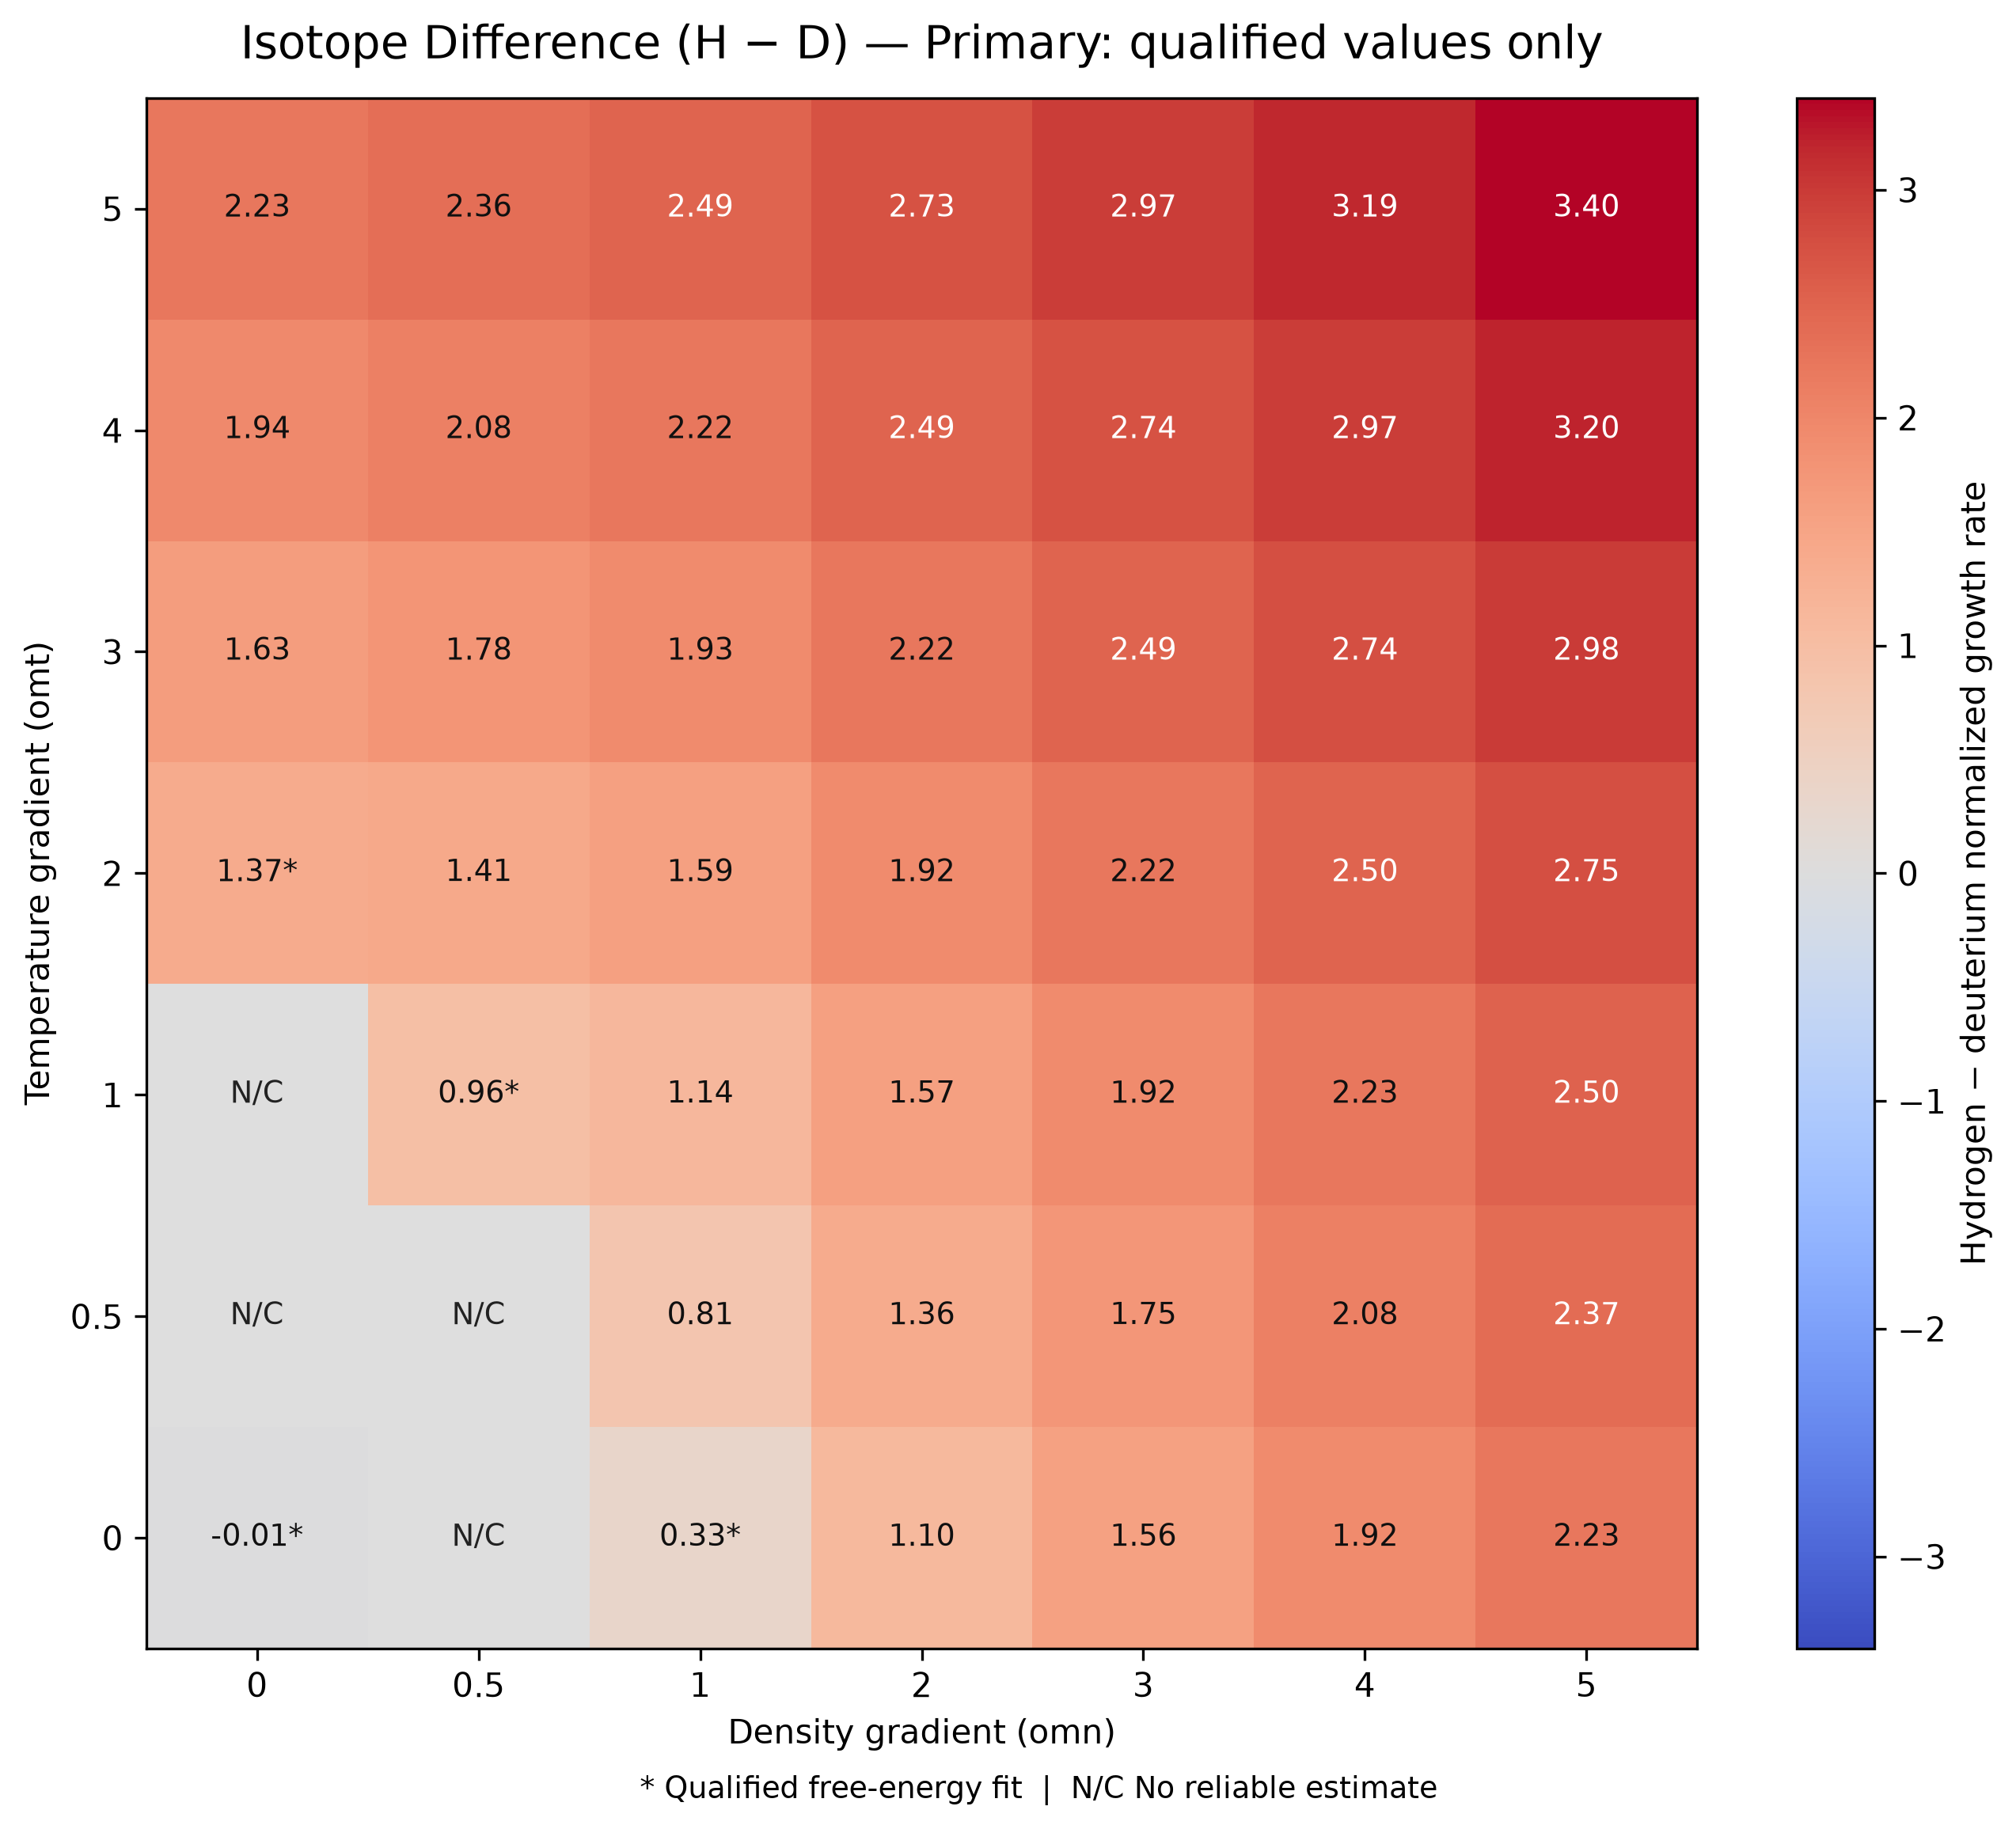
\includegraphics[width=\linewidth]{primary_validated_difference.png}
\caption{Difference, H--D}
\end{subfigure}
\caption{Primary growth-rate maps. Asterisks indicate
qualified total-free-energy estimates; gray cells
indicate cases without a reliable estimate.}
\end{figure}

In the converged region, growth rates increase
with both density and temperature gradients.
At $\mathrm{omn}=\mathrm{omt}=2$,
\[
\gamma_H=6.096,\qquad
\gamma_D=4.172.
\]
The deuterium rate is approximately 31.6\%
lower than the hydrogen rate at this point.
At $\mathrm{omn}=\mathrm{omt}=5$,
the corresponding rates are approximately
10.426 and 7.022.

All \textbf{41 parameter pairs for which both
GENE simulations formally converged} satisfy
$\gamma_H>\gamma_D$.
This establishes a consistent isotope dependence
for the simulated linear modes at the selected
wavenumber.

\subsection{Supplementary Exploratory Heatmaps}

\begin{figure}[H]
\centering
\begin{subfigure}{0.32\linewidth}
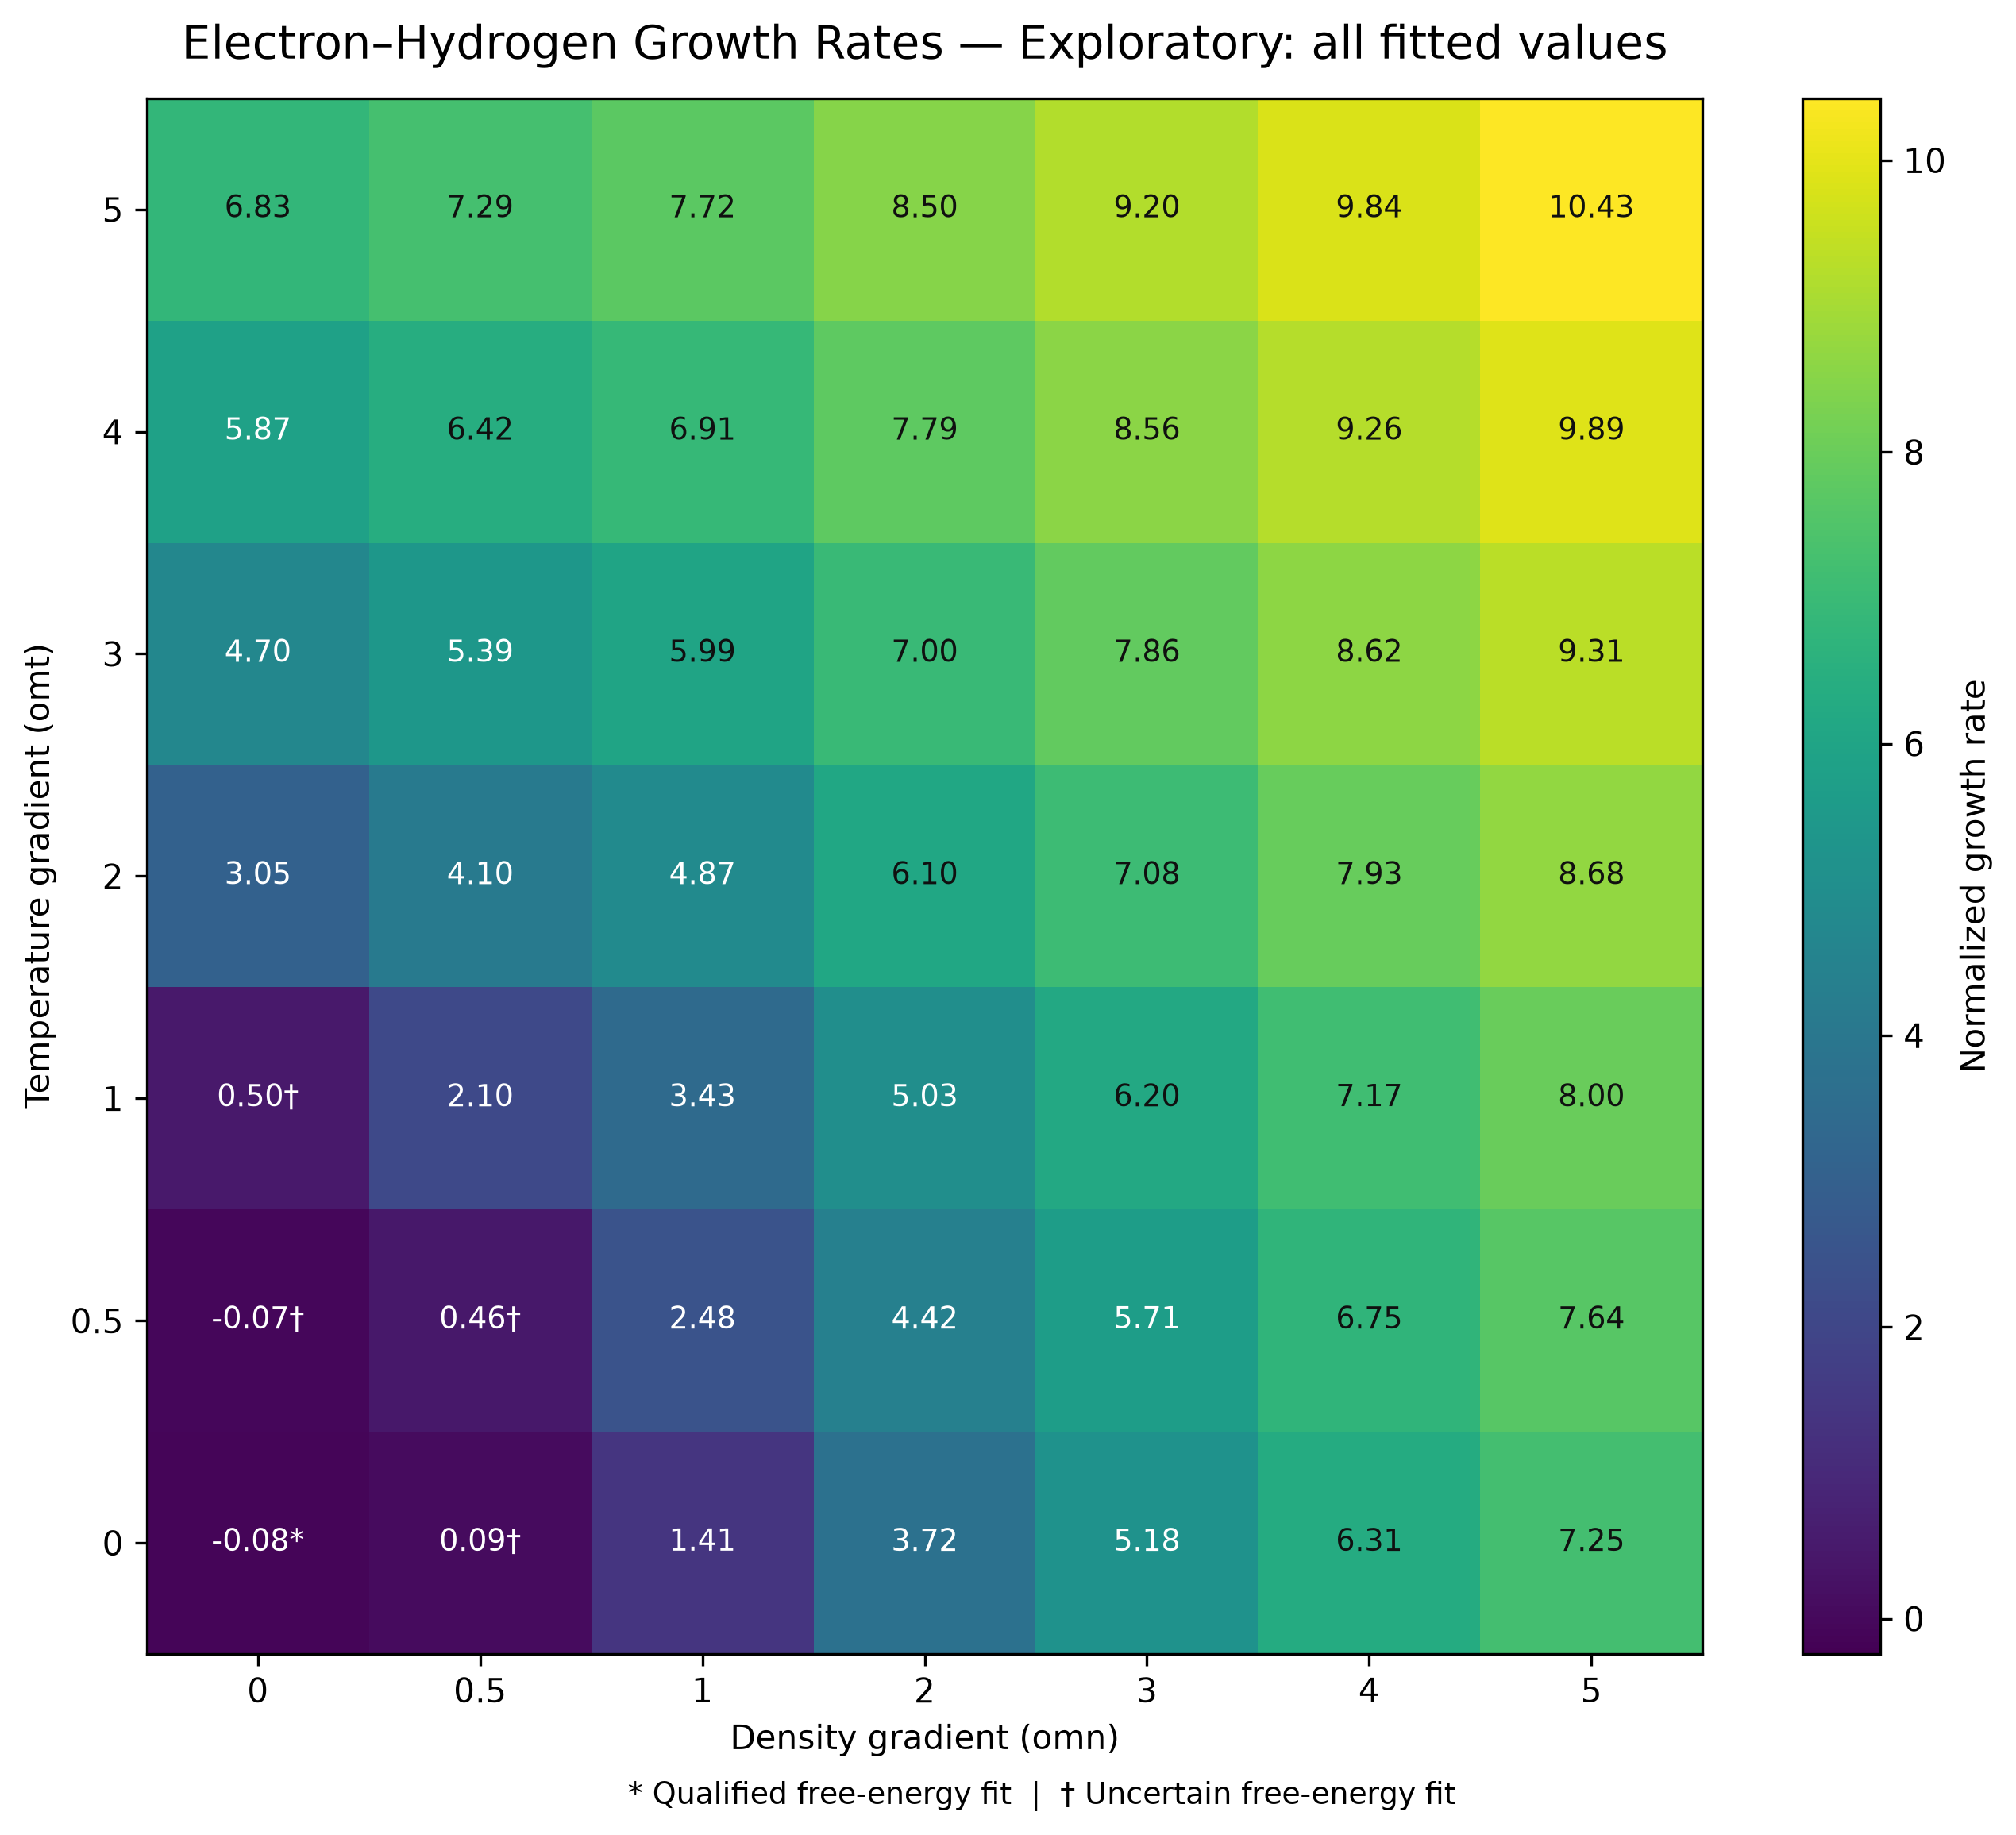
\includegraphics[width=\linewidth]{supplementary_exploratory_hydrogen.png}
\caption{Electron--hydrogen}
\end{subfigure}
\begin{subfigure}{0.32\linewidth}
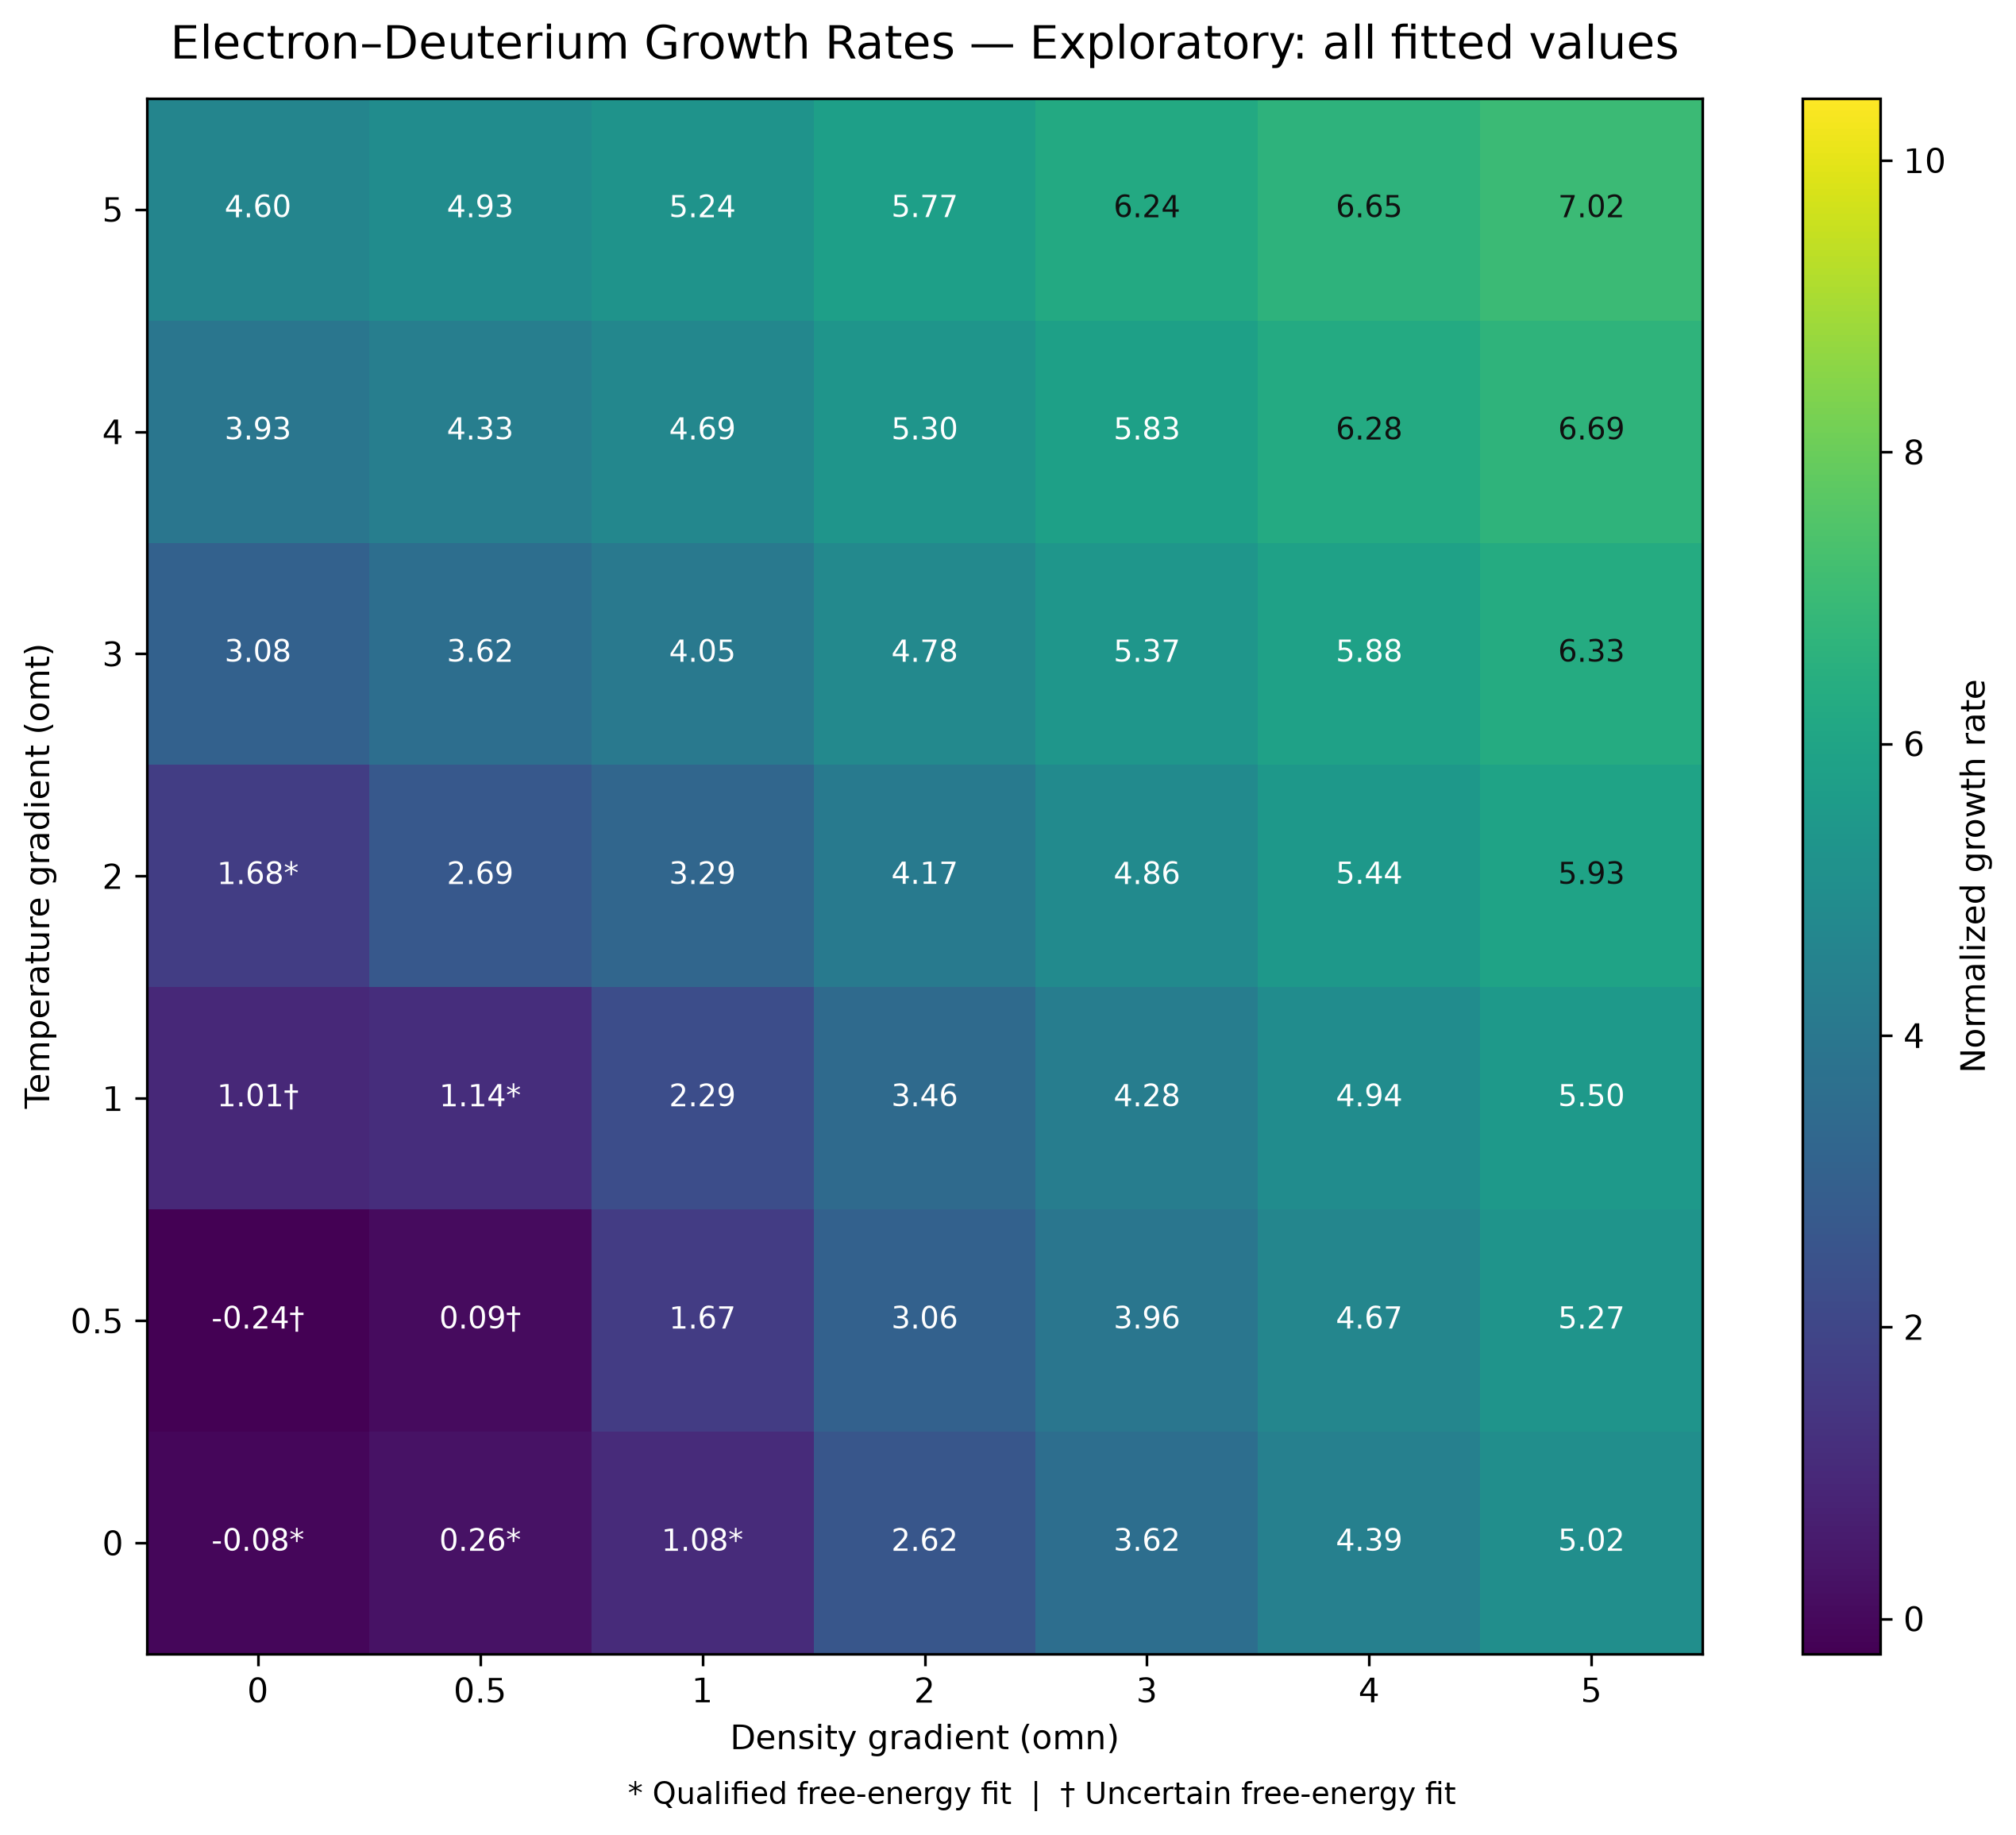
\includegraphics[width=\linewidth]{supplementary_exploratory_deuterium.png}
\caption{Electron--deuterium}
\end{subfigure}
\begin{subfigure}{0.32\linewidth}
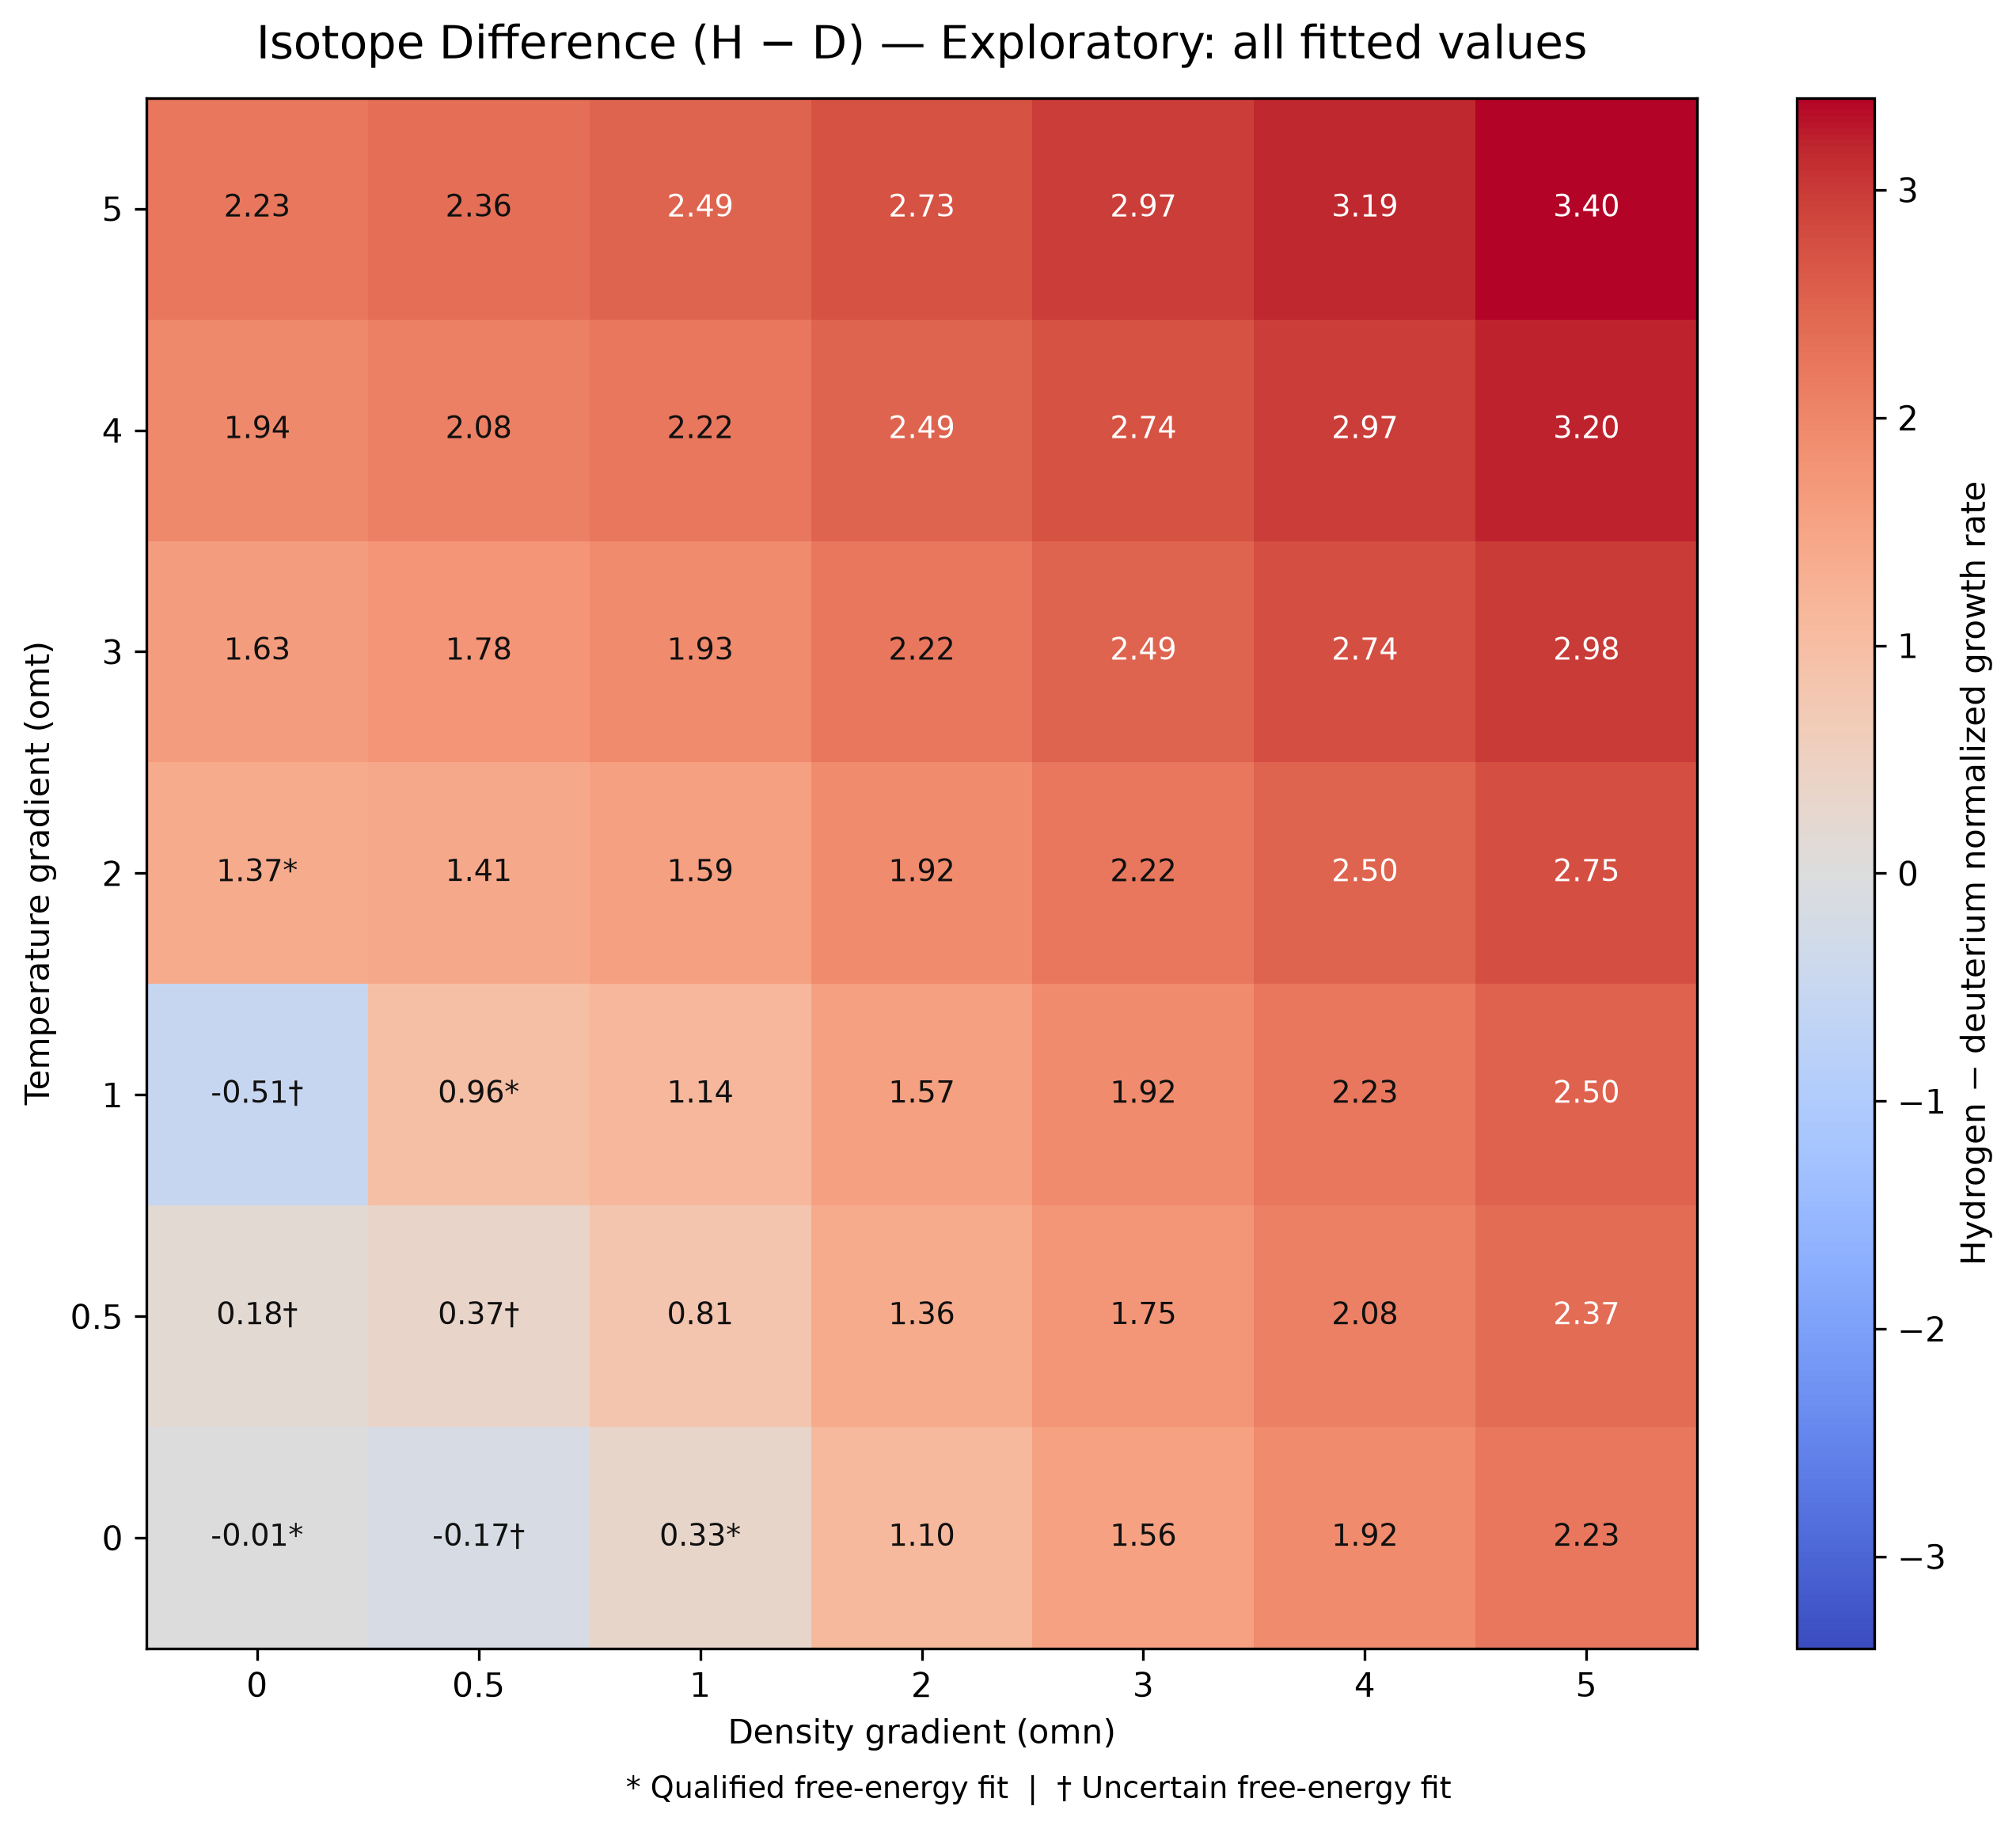
\includegraphics[width=\linewidth]{supplementary_exploratory_difference.png}
\caption{Difference, H--D}
\end{subfigure}
\caption{Exploratory maps including all energy-fit
estimates. $*$ denotes a qualified estimate and
$\dagger$ denotes an uncertain estimate.}
\end{figure}

The exploratory maps fill the low-gradient
region but reveal the sensitivity of some
results to the fitting procedure.
At $\mathrm{omn}=\mathrm{omt}=0$,
the estimated rates are approximately
$\gamma_H=-0.081$ and $\gamma_D=-0.075$.
Both negative values are consistent with
decaying total free energy.

Some uncertain low-gradient comparisons yield
$\Delta\gamma<0$, including
$\Delta\gamma\approx-0.51$ at
$(\mathrm{omn},\mathrm{omt})=(0,1)$.
Because these results depend on uncertain
energy fits, they do not establish a confirmed
reversal of the isotope trend.

\section{Conclusions and Limitations}

The 98-case scan demonstrates that stronger
density and temperature gradients are associated
with larger normalized linear growth rates in
the GENE-converged region. At fixed
$k_{y,\min}=0.7$, electron--hydrogen plasmas
consistently exhibit higher growth rates than
electron--deuterium plasmas wherever both
simulations formally converged.

The free-energy method recovered useful
late-time estimates for all 13 initially
unresolved simulations, but only six were
classified as sufficiently reliable for
the primary figures. The remaining seven
were retained as explicitly uncertain
exploratory values.

These findings concern linear stability at
one perpendicular wavenumber, not nonlinear
turbulence or confinement performance.
A separate wavenumber scan can test whether
the isotope ordering persists across the
mode spectrum. Further resolution and
convergence studies would be needed to
characterize the weak-gradient regime
more definitively.

\end{document}
